% Chapter 4

\chapter{Layout und Struktur} % Main chapter title

\label{LayoutStruktur} % For referencing the chapter elsewhere, use \ref{Chapter1}

\lhead{\chaptername{} \thechapter{} - \emph{Layout und Struktur}} % This is for the header on each page - perhaps a shortened title

%----------------------------------------------------------------------------------------

Während der Fehleranalyse konnten immer wieder grundlegende Fehler in der Anordnung von Elementen beobachtet werden, die dazu führten, dass ein Artefakt unsauber wirkte.
Diese Fehler lassen sich mit sehr simplen Mitteln, wie Hilfslinien oder Grid Systems, vermeiden.
Hier unterscheiden sich die verschiedenen Medien und Plattformen im Hinblick auf bestehende Lösungen und mögliche Ansätze, weshalb dieses Kapitel in jeweils spezifische Unterkapitel unterteilt ist.

\section{Grid Systems im Web}
Für Gestaltungen im Web sind Grid Systems sehr verbreitet, nicht zuletzt auch wegen ihres hohen Mehrwertes im Bezug auf Responsive Webdesign.
Wegen der hohen Anzahl bereits bestehender Lösungen liegt es nahe, dass das Tool dem Nutzer nicht beim Erstellen eines eigenen Grid Systems hilft, sondern nur die Grundlagen vermittelt und für die Umsetzung auf eine bereits bestehende Lösung verweist.
Hierfür wurden zunächst verschiedene Grid Systems auf ihre Konfigurationsmöglichkeiten und ihren Output hin untersucht und evaluiert.

\textbf{gridpak} (http://gridpak.com) \\
Geeignet, um individuelle Grid Systems zu erstellen. Sehr simpel, da nur drei Werte verändert werden müssen (plus Option zum Anlegen von Breakpoints). \\
\textit{Output:} Verschiedene CSS und JS Files und das Grid System als png.

\textbf{960px Grid} (http://960.gs) \\
Festes, 960px breites Grid System, keine individuellen Einstellungen mehr Möglich. \\
\textit{Output:} Verschiedene CSS Dateien sowie vorlagen für viele Grafikprogramme.

\textbf{1200px Grid} (https://1200px.com) \\
Aufbauend auf dem 960px Grid, aber 1200px breit. Außerdem in allen Werten anpassbar. \\
\textit{Output:} CSS Dateien oder Photoshop/Illustrator Files.

\textbf{Bootstrap} (http://getbootstrap.com/2.3.2/index.html) \\
Sehr flexibel und anpassbar, allerdings nur, wenn es im Web verwendet wird, Einbindung über HTML/CSS also Pflicht. \\
\textit{Output:} Im Code verwendbare CSS-Klassen.

\textbf{Dead Simple Grid} (https://github.com/mourner/dead-simple-grid) \\
Ähnlich wie Bootstrap aber sehr viel simpler. Flexibel anpassbar, aber ebenfalls nur für die Verwendung mit HTML/CSS geeignet. \\
\textit{Output:} Im Code verwendbare CSS-Klassen.

\textbf{Bourbon Neat} (http://neat.bourbon.io) \\
Ähnlich wie Bootstrap \& Dead Simple Grid aber deutlich komplexer, da es zwingen über einen CSS-Präprozessor eingebunden werden muss. Flexibel anpassbar, aber ebenfalls nur für die Verwendung mit HTML/CSS geeignet. \\
\textit{Output:} Im Code verwendbare CSS-Klassen.

\textbf{Foundation} (http://foundation.zurb.com) \\
Ähnlich wie Bootstrap. Flexibel anpassbar, aber auch nur für HTML/CSS geeignet. \\
\textit{Output:} Im Code verwendbare CSS-Klassen.

\subsection{Abbildung im Tool}
Da sich die untersuchten Grid Systems in ihren Eigenschaften sehr unterscheiden, sollte das Tool mehrere Empfehlen und ihre typischen Einsatzgebiete nennen.
Die Wahl fiel mit gridpack auf ein System, das auch unabhängig vom Code eingesetzt werden kann, sowie auf Foundation, das nur im CSS verwendet werden kann. Foundation wurde gewählt, da es die Möglichkeit bietet, nur das Grid System ohne Klassen für andere Elemente, wie zum Beispiel Buttons, einzubinden.
Um dem Nutzer das Arbeiten mit Grid Systems näher zu bringen, könnte das Tool diesen dazu auffordern, verschiedene Elemente auf einer Seite zu Platzieren. Zunächst sollte die Platzierung ohne eine Hilfestellung stattfinden (s. Abb.X), im zweiten Schritt dann mit einem simplen, vom User konfigurierten Grid System (s. Abb.X).

\section{Grid Systems auf nativen Plattformen}
Auf nativen Plattformen werden Grid Systems eher von Interface Designern verwendet, vorgefertigte Grid Systems  wie sie im Web für die Umsetzung verwendet werden können, bestehen in dieser Art nicht. Die Zielgruppe des Tools besteht jedoch nicht aus Interface Designern, sondern aus Studenten, die Projekte in der Regel in der Rolle des Entwicklers durchführen. Hier müssen also plattformspezifische Grundlagen gefunden werden.

Unter iOS spielt das Storyboard in Xcode für die Platzierung von Elementen eine wichtige Rolle. Im Storyboard ist ein implizites Grid System vorhanden, dass zumindest die Außenabstände und die Abstände von Elementen untereinander mit Hilfslinien kennzeichnet. (s. Abb. \ref{fig:xcode-guides} auf Seite \pageref{fig:xcode-guides})
Das Tool sollte an dieser Stelle auf die Verwendung des Storyboards hinweisen, eine weitere Interaktivität macht wenig Sinn.

\begin{figure}[h]
    \centering
    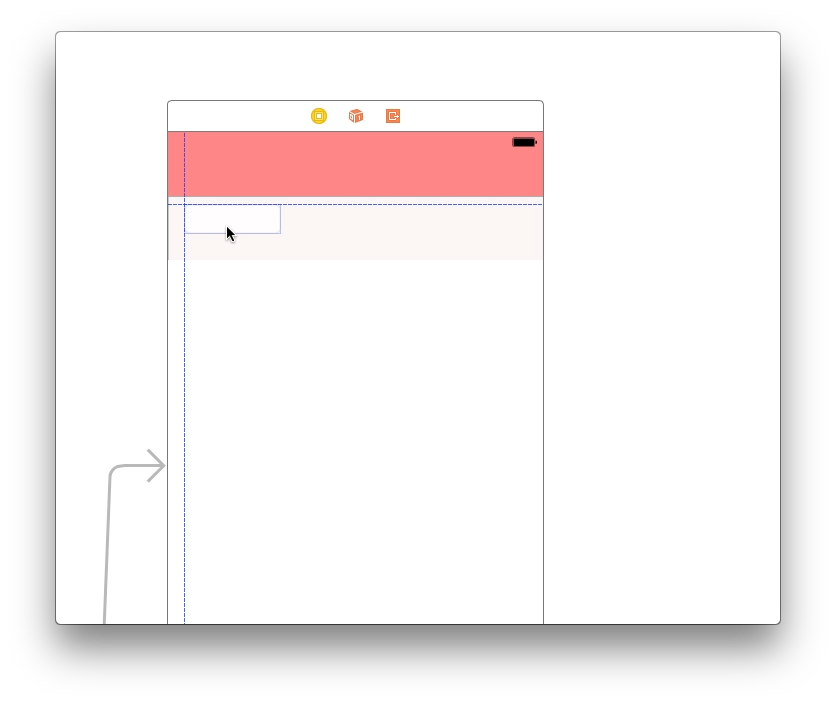
\includegraphics[width=1\textwidth]{images/xcode-guidelines.png}
    \caption{Automatische Guidelines im Xcode Stroyboard}
    \label{fig:xcode-guides}
\end{figure}

Für Android gestaltet sich das erstellen von Layouts schwieriger, da der in Android Studio enthaltene Visuelle Editor deutlich weniger intuitiv ist und weniger Hilfestellung liefert, als die Storyboards von Xcode. Das Interface wird hier in der Praxis außerdem deutlich häufiger in XML-Form beschreiben und nicht durch den visuellen Editor erzeugt. In den Material Design Guidelines wird generell ein 8dp Square Grid verwendet. Das heißt, der Abstand von allen Elementen nach außen beträgt mindestens 8dp, jedoch sind für alle UI-Elemente auch zusätzlich spezifische Abstände angegeben, auf die verwiesen werden sollte. Für alle Elemente und Endgeräte sind außerdem Illustrator-Vorlagen vorhanden. 

\section{Grid Systems in einfachen Texten}
Generell sind Grid Systeme auch im Textsatz-Bereich sehr verbreitet und finden dort sogar ihren Ursprung. Sie unterscheiden sich aber durchaus von Grid-Systemen, wie man sie im Web-Bereich verwendet. Auch hier gibt es verschiedene Ausführungen, so werden horizontale Raster verwendet, um die Ausrichtung der Zeilen über die Seite hinweg zu ordnen oder der Satzspiegel, der die harmonische Platzierung von Text auf einer Doppelseite vereinfacht. \\
Das Tool soll sich aber auf Systeme konzentrieren, die nur wenige Spalten als Platz für den Fließtext verwenden.

Da viele der im Rahmen der Fehleranalyse untersuchten Artefakte einzelne Textseiten (beispielsweise Exposés) waren, wird der Fokus des Tools darauf liegen, eine einzelne Textseite zu setzen.
Hier sind sowohl die Abstände vom Text zum Rand der Seite als auch die Abstände von Spalten untereinander interessant.

Weiterhin sollte erwähnt werden, dass die meisten Textverarbeitungsprogramme diese Abstände bereits in den Standardeinstellungen auf solide Werte setzen und das Tool auch hier eher ein Grundverständnis vermitteln, als eine konkrete Lösung anbieten sollte.

\subsection{Berechnung}
Die simpelste mögliche Berechnung verwendet einen Bruchteil der Gesamtlänge der kürzesten Kante des Dokumentes als Außenabstand. Für ein DIN A4 Blatt mit einer Breite von 595px oder 210mm ergibt sich bei der Verwendung von 10\% der Breite ein Außenabstand von etwa 60px oder 21mm.
Eine so gesetzte Textseite kann Abb. \ref{fig:a4-single-col} auf Seite \pageref{fig:a4-single-col} entnommen werden.

\begin{figure}[h]
    \centering
    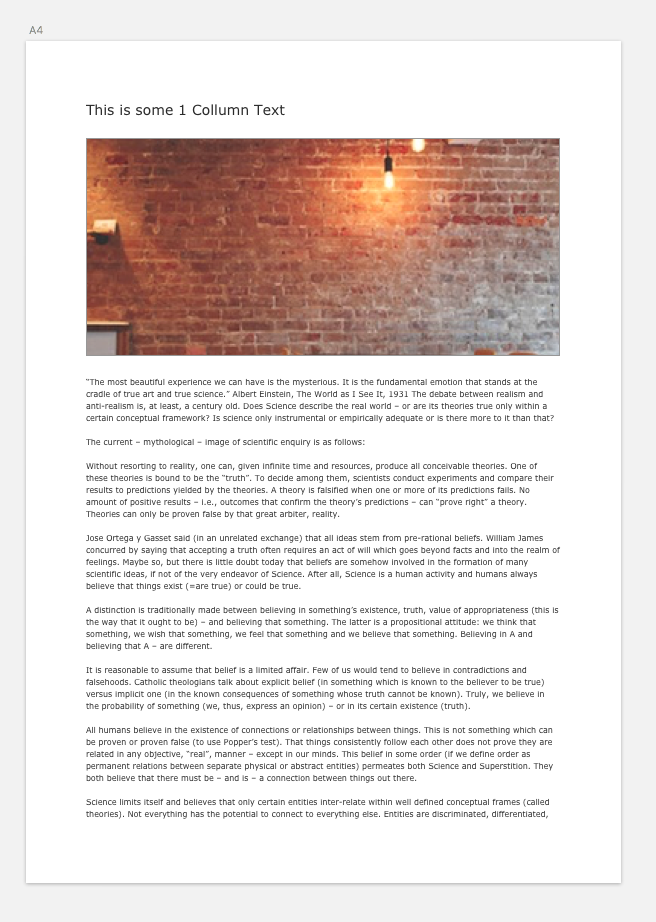
\includegraphics[width=0.5\textwidth]{images/A4-single-col.png}
    \caption{Mit 10\% außenabstand gesetzte DIN-A4 Seite}
    \label{fig:a4-single-col}
\end{figure}

Mit diesem Wert ist zunächst also eine grobe Richtlinie gefunden. Nach unten lassen sich für den Abstand genaue Grenzen finden: Viele Drucker benötigen einen Druckrand von etwa 15mm, das Tool sollten den Nutzer also warnen, sollte der Abstand nach außen diesen Wert unterschreiten.

Sollte ein Layout mit mehr als einer Spalte gewünscht sein, kann der Abstand zwischen diesen Spalten ebenfalls über den errechneten Außenabstand definiert werden. Der Abstand zwischen den Spalten sollte dabei kleiner sein, als der nach außen, es bietet sich also die Hälfte des Außenabstandes an. Mit den oben errechneten Werten wäre der Abstand zwischen zwei Spalten also 30px oder etwa 10mm. Ein mit diesen Werten gesetzter Text kann Abb. \ref{fig:a4-two-col} auf Seite \pageref{fig:a4-two-col} entnommen werden.

\begin{figure}[h]
    \centering
    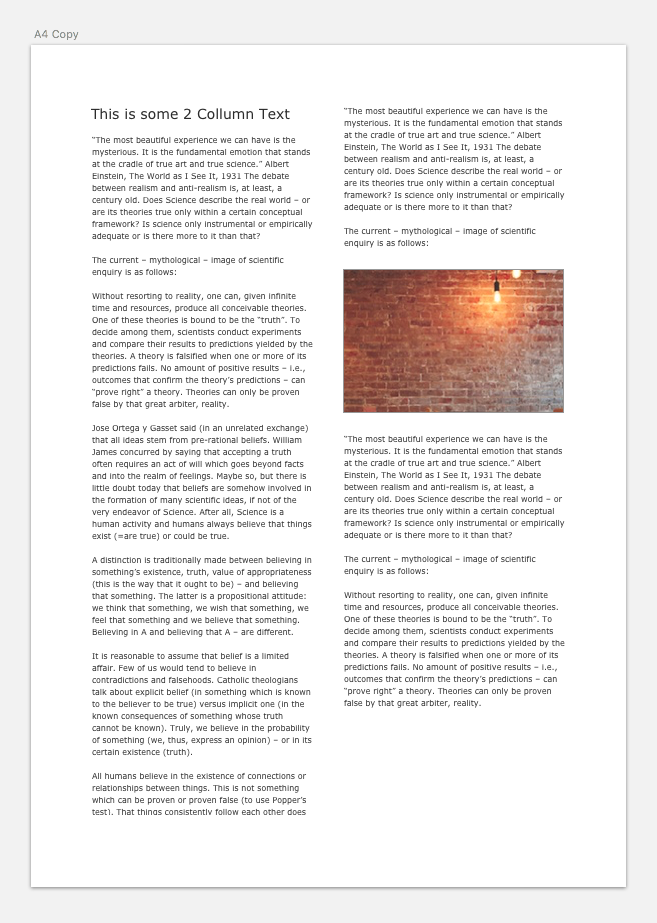
\includegraphics[width=0.5\textwidth]{images/A4-two-col.png}
    \caption{Eine mit zwei Spalten Text und 30px Abstand gesetzte DIN-A4 Seite}
    \label{fig:a4-two-col}
\end{figure}

Zu beachten ist hier, dass die Spalten mit diesen Werten nur jeweils 445px breit wären und hierdurch die im Kapitel Typographie behandelte optimale Laufweite des Textes von 75 - 90 CPL je nach verwendeter Schriftgröße nicht mehr gewährleistet ist. Das Tool sollten die im ersten Schritt errechneten Werte für Texte kennen und den Nutzer auf diesen Umstand hinweisen.

\subsection{Abbildung im Tool}
Das Tool soll dem Nutzer die Möglichkeit geben, ein Format zu wählen. Für dieses Format sollte der User dann die Anzahl der Spalten, die Abstände zwischen den Spalten und die Abstände nach außen einstellen können.
Das Tool weist den Nutzer dann darauf hin, welche Werte aus welchen Gründen kritisch sind.
Optional soll noch ein Bild eingefügt werden können. Die Platzierung soll dem Nutzer überlassen werden und ihn dazu bringen, bereits im Tool auch aktiv mit einem Layout zu arbeiten.
